\centering
\texttt{{\Huge О правильных многоугольниках,  \\ функции Эйлера и числах Ферма}}
\\
\texttt{{\large А.КИРИЛЛОВ}}

\begin{multicols}{3}

\noindent\rule{0.33\textwidth}{0.4pt}
\textbf{\large{Пролог}}
\noindent\rule{0.33\textwidth}{0.4pt}

\justifying
\lettrine[lines=3,nindent=2pt]{З}{}АДАЧИ на геометрические по-
строения - одни из самых по-
пулярных в школьной математике
Почти в каждом математическом
кружке разбираются такие задачи.
Это, конечно, не случайно. История
геометрических построений насчиты-
вает несколько тысяч лет, и уже
древние греки достигли здесь боль-
шого искусства. В качестве примера
можно привести задачу Аполлония:
\textit{построить окружность,  касающуюся трех данных окружностей.}

Многим,  вероятно,  известны три \\
знаменитые задачи древности,  ока-
завшиеся неразрешимыми: \textit{о квад-
ратуре круга, трисекции угла и
удвоении куба}.

Но, пожалуй, самой красивой яв-
ляется задача о построении правиль-
ных многоугольников. Собственно го-
воря, это не одна задача, а целая
серия задач: \textit{для каждого натураль-
ного числа n $\geq$ 3 требуется с по-
мощью циркуля и линейки построить правильный n-угольник}.

Для некоторых значений n эта зада-
ча совсем простая (например, для n =
= 3, 4, 6, 8, 12); для других – послож-
нее (n = 5, 10, 15; ниже мы расска-
жем, как построить десятиугольник и
пятиугольник); для третьих - очень
сложная (n = 17 или 257).  Наконец,
существуют такие значения n, для
которых эта задача вообще неразре-
шима (например, n = 7, 9, 11).

Выпишем подряд несколько нату-
ральных чисел, начиная с n = 3, и
Отметим красным цветом те числа n,
для которых можно построить пра-
\columnbreak
\\
«черных» чисел? Оказывается, есть;
но найти её довольно трудно. Эта за-
кономерность имеет арифметическую
природу, чтобы ее описать, нам при-
дется временно оставить геометрию и
заняться элементами теории чисел -
высшего раздела арифметики.

\noindent\rule{0.33\textwidth}{0.4pt}
\textbf{\large{Функция Эйлера}}

\noindent\rule{0.33\textwidth}{0.4pt}
Важной арифметической характерис-
тикой числа n является количество 
чисел, меньших n и взаимно простых
с n.  Одним из первых это заметил 
знаменитый математик XVIII века
Леонард Эйлер. Он предложил для
этого количества обозначение $\varphi(n)$, и
с тех пор функция $n \to \varphi(n)$ известна
под именем \textit{«функции Эйлера»}. На-
пример, для n = 10 имеется четыре 
числа,  меньших десяти и взаимно про-
стых с ним: 1, 3, 7 и 9; так что \\
$\varphi(10) = 4.$

Функция $\varphi$ обладает многими ин-
тересными свойствами.  Одно из них
было открыто ещё самим Эйлером: \\
для любых двух взаимно простых
чисел m и n справедливо равенство: \\
\begin{equation}
\varphi(mn) = \varphi(m)\varphi(n).
\end{equation}

Кроме того, легко проверить, что
\textit{если р - простое ҹисло,  то \\
$\varphi(p) = p - 1,  \varphi(p^2) = p^2 - p$,  и вообще}
\begin{equation}
\varphi(p^m) = p^{m - 1}(p - 1).
\end{equation}

Эти свойства позволяют легко вы-
числять функцию Эйлера для не-
больших значений n.  Например,
$$\varphi(10) = \varphi(2)\cdot\varphi(5) = 1\cdot4 = 4,$$
\columnbreak
$$\varphi(100) = \varphi(4)\cdot\varphi(25) = 2\cdot20 = 40.$$

Мы приводим здесь значения фун-
кции Эйлера для n от 1 до 42 (см.
таблицы 1,  \textit{а} и \textit{б}).

Сравните эти таблицы с приведен-
ным выше рядом «красных» и «чер-
ных» чисел.  Не правда ли, связь
между «цветом» чисел n и значением
$\varphi(n)$ уже легко угадывается? Мы
видим, что если правильный n-уголь-
ник можно построить с помощью
циркуля и линейки,  то соответствую-
щее значение функции ф(n) является
степенью двойки.  Оказывается, это
условие является необходимым и
достаточным для возможности пос-
троения правильного n-угольника.

В настоящей статье мы не сможем
строго доказать это.  Однако мы приведем достаточно простые и 
убедительные соображения в пользу этого
факта.  Аналогичные соображения
применимы и ко многим другим задачам на построение - например,  к
задаче о трисекции угла.
\noindent\rule{0.33\textwidth}{0.4pt}
\textbf{\large{Что значит «построить»?}}

\noindent\rule{0.33\textwidth}{0.4pt}
Вопрос о точной постановке задач на
построение циркулем и линейкой уже
обсуждался на страницах «Кванта».
Мы не будем здесь еще раз предос-
терегать читателей от неправильного
употребления математических ин-
струментов.  Скажем лишь, что окон-
чательное решение задачи на построе-
ние должно быть (хотя бы в принципе)
записываемо в виде цепочки элемен-
тарных операций, напоминающей сис-
тему команд,  отдаваемых электрон-
ной вычислительной машине.

\end{multicols}
\vspace*{-\baselineskip}
\vspace{1mm}

\begin{vwcol}[widths={0.32,  0.67},  sep=.8cm,  justify=flush,  rule=0pt,indent=0em]
\justifying
вильный n-угольник циркулем и ли-
нейкой:
\\
3, 4, 5, 6, 7, 8, 9, 10, 11, 12, 13, 14,
15, 16, 17, 18, 19, 20, 21, 22, 23, 24,
25, 26, 27, 28, 29, 30, 31, 32, 33, 34,
35, 36, 37, 38, 39, 40, 41, 42, 43, 44,
45, 46, 47, 48...

Есть ли какая-нибудь закономер- \\
ность распределении «красных» и \\
\noindent\rule{3cm}{1pt} \\
\textit{\small \phantom{..}Эта статья впервые была опубликована в "Кванте" № 7 за 1977 год.}

\phantom{....}

\raggedleft
\textbf{\textit{Таблица 1,  a}}

\phantom{....}

\raggedright
\begin{tabular} { 
	| m{1.5em} | m{4pt} | m{4pt} | m{4pt} |  m{4pt} | m{4pt} | m{4pt} | m{4pt} | m{4pt} | m{4pt} | 
	m{5pt} | m{5pt} | m{5pt} | m{5pt} | m{5pt} | m{5pt} | m{5pt} | m{5pt} | m{5pt} | m{5pt} | m{5pt} | m{5pt} |
}
 \hline
 n & 1 & 2 & 3 & 4 & 5 & 6 & 7 & 8 & 9 & 10 & 11 & 12 & 13 & 14 & 15 & 16 & 17 & 18 & 19 & 20\\
 \hline
 $\varphi(n)$ & 1 & 1 & 2 & 2 & 4 & 2 & 6 & 4 & 6 & 4 & 10 & 4 & 12 & 6 & 8 & 8 & 16 & 6 & 18 & 8\\
\hline
\end{tabular}

\phantom{....}

\phantom{....}

\raggedleft
\textbf{\textit{Таблица 1,  б}}

\phantom{....}

\raggedright
\renewcommand{\tabcolsep}{5.5pt}
\begin{tabular} { 
	| m{1.37em} | m{4.5pt} | m{4.5pt} | m{5pt} | m{4.5pt} | m{5pt} | m{5pt} | m{4.5pt} | 
	 m{5pt} | m{5pt} | m{5pt} | m{4pt} | m{4.5pt} | m{5pt} |  m{4.5pt} | m{5pt} | 
	 m{5pt} | m{5pt} | m{5pt} | m{5pt} | m{5pt} | m{4.5pt} | m{4.5pt} | 
}
 \hline
 n & 21 & 22 & 23 & 24 & 25 & 26 &27 & 28 & 29 & 30 & 31 & 32 & 33 & 34 & 35 & 36 & 37 & 38 & 39 & 40 & 41 & 42\\
 \hline
 $\varphi(n)$ & 12 & 10 & 22 & 8 & 20 & 12 & 24 & 12 & 28 & 8 & 30 & 16 & 20 & 16 & 24 & 12 & 36 & 18 & 24 & 16 & 40 & 12\\
\hline
\end{tabular}
\end{vwcol}

\newpage

\centering
\texttt{{\large К В А Н Т  $\cdot$ 1 9 9 4 / № 6}}

\begin{multicols}{3}
\justifying
Натример, задача о построении
середины отрезка AB решается сле-
дующей программой» (рис.1):
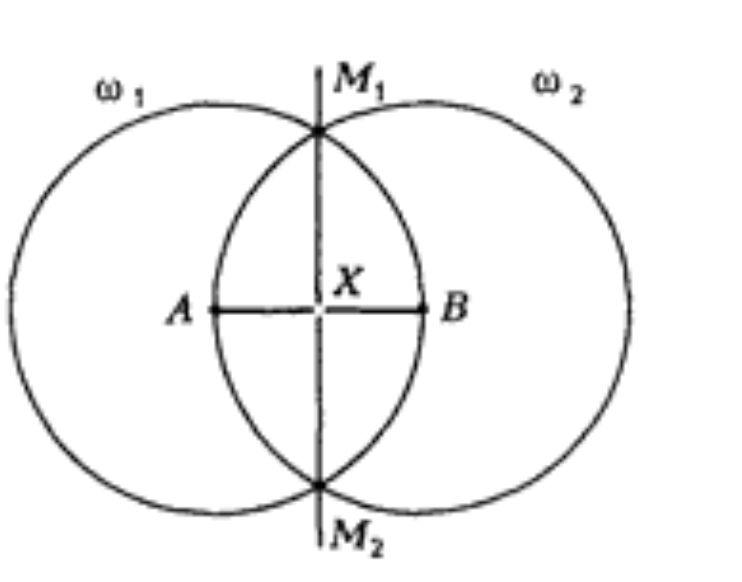
\includegraphics[width=0.29\textwidth]{circles1}
\raggedright
\textbf{Рис.  1}

\begin{enumerate}
\item \small \textit{Циркулем построить окружность $\omega_1$ с центром A и радиусом AB.}
\item \small \textit{Циркулем построить окружность $\omega_2$ с центром В и радиусом BA.}
\item \small \textit{Отметить точки пересечения $M_{1}$,  и 
$M_{2}$ окружностей $ \omega_{1}$ и $\omega_{2}$.}
\item \small \textit{По линейке провести прямую $M_{1}M_{2}$.  \\}
\item \small \textit{Отметить точку Х пересечения прямых $M_{1}M_{2}$,  и AB.}
\end{enumerate}

\justifying
Еще один пример: построение бис-
сектрисы заданного угла лов
(рис.2). Соответствующая система
команд имеет вид:

\columnbreak
имеет с прямыми ОА и ОВ по две
точки пересечения, и неясно, какие
из этих точек нужно обозначить че-
рез А, и В.  Вы можете возразить,
что речь идет о лучах ОА и ОВ,
которые пересекаются с окружностью
в единственной точке, но понятие
«луч» выходит за рамки понимания
нашей «математической машины» ‚ Ей
доступно только понятие «прямая».

Посмотрим, что получится, если
понимать выражение «точка пересе-
чения» как «какая-нибудь точка пе-
ресечения». Тогда нашей программе
будет соответствовать рисунок 3: вмес-

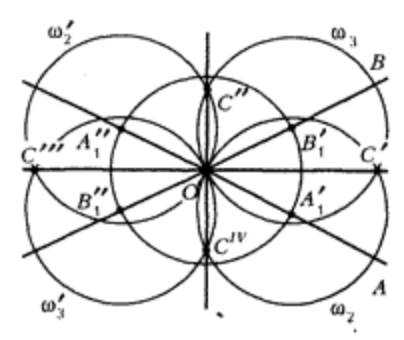
\includegraphics[width=0.29\textwidth]{circles2}
\raggedright
\textbf{Рис.  3}

\columnbreak
выполнение этой операции приводит
к двум реализациям (как в разобран-
ном выше примере). Вообще, если в
программе есть k двузначных опера-
ций, то эту программу можно реали-
зовать $2^k$ способами.

Мы видели, что некоторые неопре-
деленности могут в конце концов «со
кращаться» и не влиять на окончатель-
ный ответ. Оказывается (это можно
строго доказать, но не в этом цель
настоящей статьи), такие сокращения
всегда происходят согласованным об-
разом, так что неопределенность в
окончательном ответе всегда имеет вид
$2^l (l \leq k)$. Этот факт имеет не геомет-
рическую, а алгебраическую природу
(соответствующая часть алгебры на-
зывается теорией Галуа).

Вернемся к задаче о построении
биссектрисы. Наша программа, кро-
ме биссектрисы угла АОВ, дает так-
жеибиссектрису внешнего угла АОВ,
(см. рис.3). Это решение не надо
рассматривать как «постороннее». С
точки зрения циркуля и линейки,
«понимающих» угол только как пару
пересекающихся прямых, этот угол
ничем не хуже исходного угла АОВ.
Попробовав определить понятие бис-
сектрисы в терминах, «доступных»
циркулю и линейке, мы увидим, что
\end{multicols}